According to \hyperref[acro:VISOR]{VISOR}\textsuperscript{\textregistered} \cite[page 22]{visor_user_manual} user manual, the \hyperref[acro:VISOR]{VISOR}\textsuperscript{\textregistered} vision sensor is an optical sensor and is used for the non-contact acquisition or identification of objects.
The vision sensor features a number of different evaluation methods (detectors), with the specific methods
depending on the specific model sensor. The product is designed for industrial use only. The \hyperref[acro:VISOR]{VISOR}\textsuperscript{\textregistered} vision sensor is a cost-effective alternative to conventional image processing systems.


\begin{figure}[h]
    \centering
    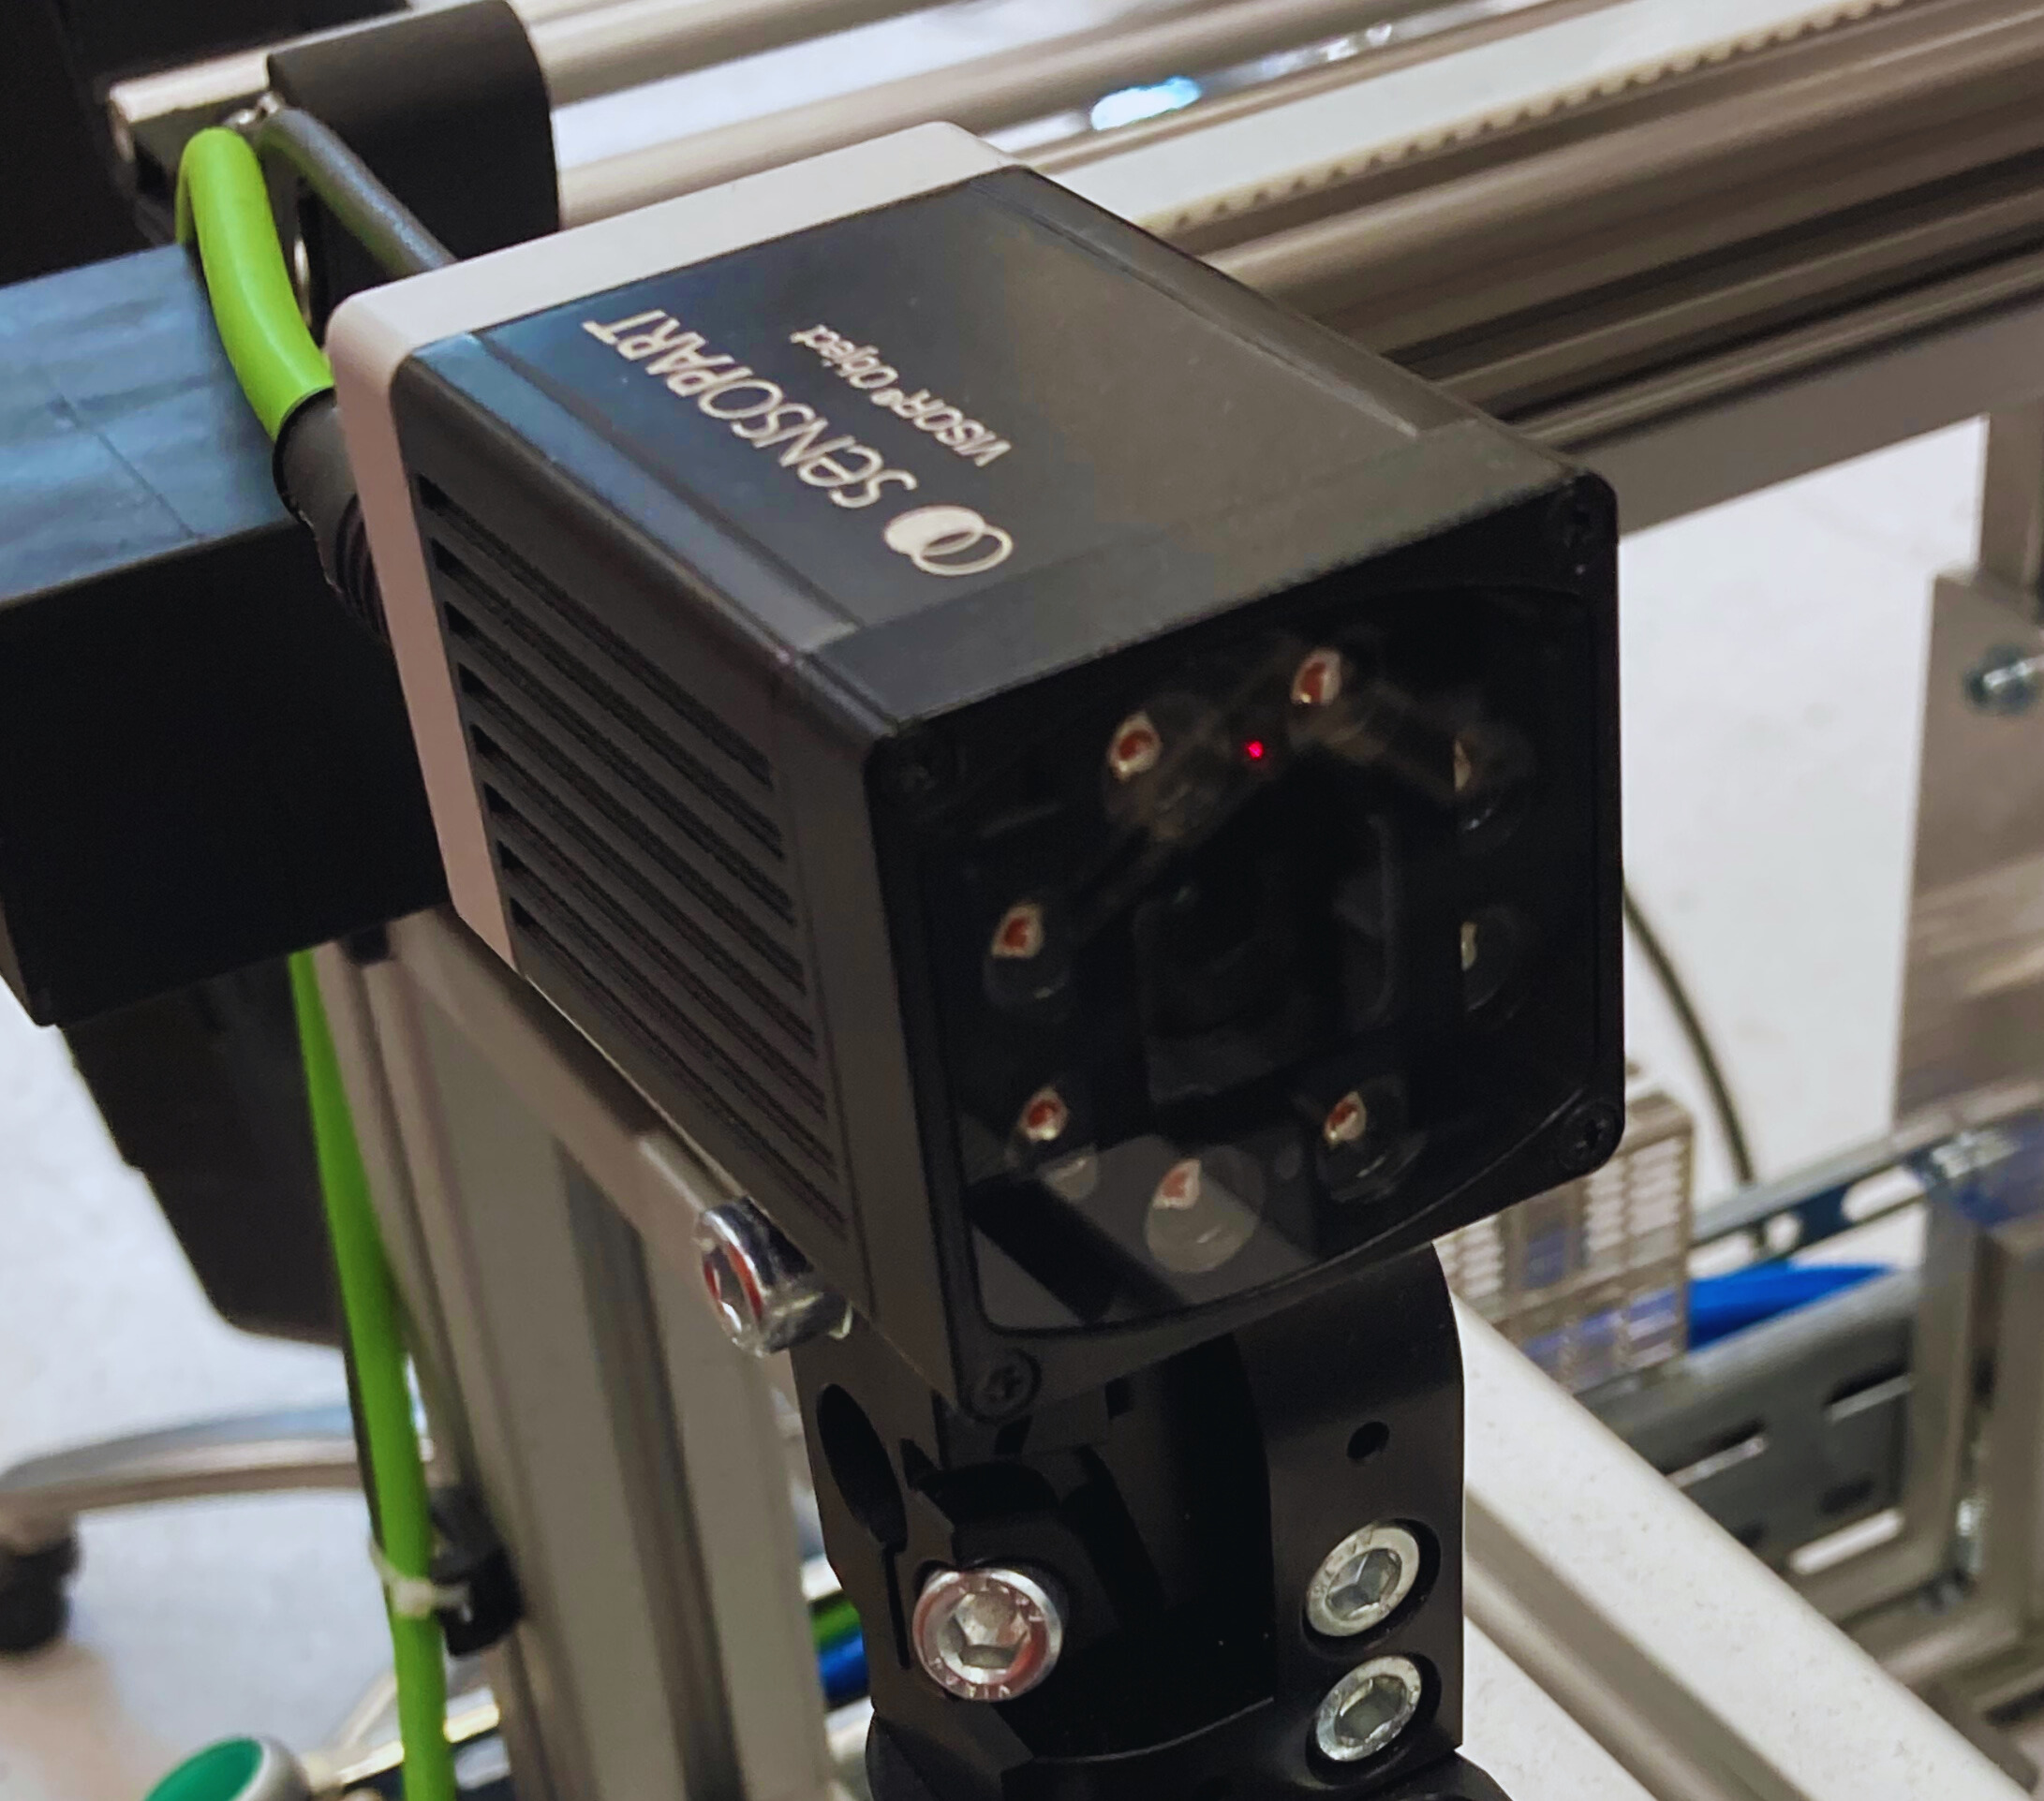
\includegraphics[width=0.4\textwidth]{figures/vision-sensor.png}
    \caption{\hyperref[acro:VISOR]{VISOR}\textsuperscript{\textregistered} vision sensor}
    \label{fig:vision-sensor}
\end{figure}

\hyperref[acro:VISOR]{VISOR}\textsuperscript{\textregistered} vision sensor is a suitable choice for the identification and classification of metal sheets for the automated bending process.
These sensors enable precise detection and processing of features on sheets, which leads to the efficiency and accuracy of automated bending process.
Special considerations need to be taken in complex industrial environments, where light reflections or changing extraneous light can distort evaluation results. For this reason, an external light source is used to protect against ambient light.

\subsubsection{Robotic Camera}
\label{subsubsec:robotic-camera}

\subsubsection{Inspection Camera}
\label{subsubsec:inspection-camera}